\documentclass[../main]{subfiles}

\begin{document}

\section{Common Inorganic Reactions}

	\subsection{Precipitate Solubility}

		\subsubsection{Table of Solubilities}


		\begin{center}
			\begin{tabular}{|r|c|c|c|c|l|}
			\hline
			\multicolumn{1}{|l|}{}                           & Group 1,       & \ch{Hg+},                                         &                                                                          & \ch{Ba^{2+}},                       & \multicolumn{1}{c|}{Else} \\
			\multicolumn{1}{|l|}{}                           & \ch{NH4+}      & \ch{Ag+}                                          & \multirow{-2}{*}{\ch{Pb^{2+}}}                                           & \ch{Ca^{2+}}                        & \multicolumn{1}{c|}{}     \\ \hline
			\ch{NO3-}                                        & \multicolumn{5}{c|}{1. All nitrates are soluble}                                                                                                                                                                \\ \hline
			\ch{X-}                                          & 2. All Group 1 & \multicolumn{2}{c|}{\cellcolor[HTML]{000000}{\color[HTML]{FFFFFF} 3. Halides of Hg, Ag and Pb are insoluble}}                & \multicolumn{1}{l|}{}               &                           \\ \cline{1-1} \cline{3-6} 
			\ch{SO4^{2-}}                                    & and ammoniums  & \multicolumn{1}{l|}{}                             & \multicolumn{2}{c|}{\cellcolor[HTML]{000000}{\color[HTML]{FFFFFF} 4. Sulfates of Pb, Ba and Ca are insoluble}} &                           \\ \cline{1-1} \cline{3-6} 
			\ch{OH-}, \ch{CO3^{2-}}, \ch{PO4^{2-}}, \ch{S2-} & are soluble    & \multicolumn{4}{c|}{\cellcolor[HTML]{000000}{\color[HTML]{FFFFFF} 5. Most other salts are insoluble}}                                                                                          \\ \hline
			\end{tabular}
		\end{center}

		\subsubsection{\usub{K}{sp} Comparison}

	\subsection{Acid/Base Reactions}

		\subsubsection{Acid/Base Titration Indicators}

		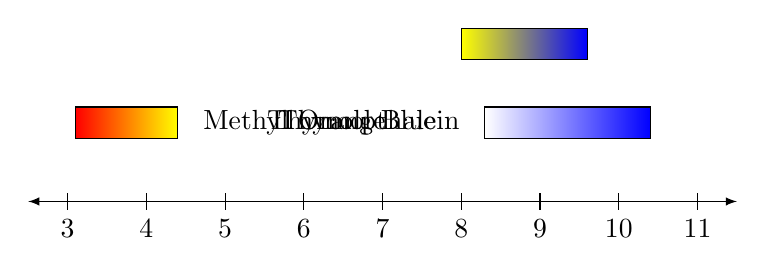
\begin{tikzpicture}
		
		\draw[left color=red, right color=yellow] (3.1,1.2) rectangle (4.4,0.8) ; 
		\draw (4.6,1) node[anchor=west] {Methyl Orange};

		\draw[left color=white, right color=blue] (8.3,1.2) rectangle (10.4,0.8) ; 
		\draw (8.1,1) node[anchor=east] {Thymolpthalein};

		\draw[left color=yellow, right color=blue] (8.0,2.2) rectangle (9.6,1.8) ; 
		\draw (7.8,1) node[anchor=east] {Thymol Blue};

		% Axis
		\draw[latex-latex] (2.5,0) -- (11.5,0) ;
		\foreach \x in  {3,4,5,6,7,8,9,10,11}
		\draw[shift={(\x,0)},color=black] (0pt,3pt) -- (0pt,-3pt);
		\foreach \x in {3,4,5,6,7,8,9,10,11}
		\draw[shift={(\x,0)},color=black] (0pt,0pt) -- (0pt,-3pt) node[below] {$\x$};
		\end{tikzpicture}

	\subsection{Redox Reactions and Reagents}

		\begin{description}
		\item[\ch{KMnO4}] is a strong oxidizing agent which will turn from purple to colorless \ch{Mn^{2+}}. Brown ppt of \ch{MnO2} forms when insufficient acid is present.
		\item[\ch{K2Cr2O7}] is a strong oxidizing agent which will turn from orange to green \ch{Cr^{3+}}.
		\item[\ch{KI}] is a reducing agent which may turn from colorless to brown \ch{I2}, possibly reducing \ch{Fe^{3+}} to form brown solution and reducing \ch{Cu^{2+}} to form cream ppt of \ch{CuI}. Use starch solution to tell if \ch{I2} is present in small concentrations, alternatively use (starchy) waste paper.
		\item[\ch{O2}] in air can oxidize:
		\begin{itemize}
			\item green \ch{Fe^{2+}} solution to brown \ch{Fe^{3+}} solution
			\item green \ch{Fe(OH)2} ppt to brown \ch{Fe(OH)3} ppt
			\item off-white \ch{Mn(OH)2} ppt to brown \ch{MnO2} ppt; and
			\item white \ch{BaSO3} ppt soluble in acid to white \ch{BaSO4} ppt insoluble in acid.
		\end{itemize}
		\item[\ch{H2O2}] can either act as a reducing agent to form \ch{H2O}, oxidizing agent (vs \ch{Fe^{2+}}) to form \ch{O2} or spontaneously decompose to form both, especially in presence of a transition metal catalyst.
		\end{description}

\end{document}
